%! Author = cnatzke
%! Date = 05/24/2022
\documentclass[cnatzke_thesis_proposal.tex]{subfiles}
\usepackage{amssymb}
\begin{document}

The interaction between radiation and materials changes depending on the charge, energy, and type of radiation involved. There are many types of radiation emitted by unstable nuclei (such as $\beta$ particles, $\alpha$ particles, protons, neutrons, $\gamma$-rays, and conversion electrons) but this section will focus on the interaction of $\beta$ particles and $\gamma$-rays via methods relevant to two-photon decay.

%------------------------------------------
\subsection{Charged Particles}
%------------------------------------------
Charges particles interact will matter primarily through the Coulomb interaction. Heavier charged particles can have many simultaneous reactions with the electrons in the impacted material diminishing the kinetic energy of the incident particle extremely rapidly, leading to a small penetration depth, whereas lighter charged particles have fewer simultaneous reactions and lose their energy more slowly creating larger penetrations depths. 

In the $\beta^-$ decay process electrons are emitted at energy ranging from a few keV to tens of MeV. Often after $\beta$-decay occurs the daughter nucleus is left in an excited state and primarily deexcites through $\gamma$-ray emission. If the $\gamma$-ray has more than 1022 keV of energy the $\gamma$-ray can undergo pair-production and produce a positron-electron pair within the field of the nucleus. The atom can also emit conversion electrons to transition to a less excited state. Regardless of the production method the interactions between the light charged particles and matter will be the same.

%------------------------------------------
\subsubsection{Bremsstrahlung Radiation}
\label{sec:bremsstrahlung_radiation}
%------------------------------------------
The emitted light charged particle will undergo multiple interactions with the electrons inside the material and with each interaction reduce the total energy of the incident particle and generally releasing Bremsstrahlung radiation.
Bremsstrahlung radiation, also called breaking radiation, is the radiation emitted by charged particles when undergoing acceleration. 
Electrons emitted via $\beta$ decay interact with atomic electrons via Coulomb scattering and will suffer large deflections and erratic behavior partly due to their relativistic speeds.
In fact the energy transfer is sufficiently large that the incident and deflected electrons become indistinguishable post collision, and the rapid changes in direction and magnitude of velocity necessitates the radiation of electromagnetic energy~\cite{krane_introductory_1987}.
The emitted radiation is called bremsstrahlung radiation. 
The energy loss per unit length for the electons can be written as: 

\begin{align}
    \left(\frac{dE}{dx}\right)_c ={}& \alpha \frac{2 \pi N_0 Z \rho}{m c^2 \beta^2 A} \left[ \ln \frac{T(T + m c^2)^2 \beta^2}{2 I^2 m c^2} + (1 - \beta^2) - (2\sqrt{1 - \beta^2} - 1 + \beta^2) \ln2 + \frac{1}{8}(1 - \sqrt{1 - \beta^2})^2 \right] \\
    \left(\frac{dE}{dx}\right)_r ={}& \alpha \frac{Z^2 N_0 (T + m c^2) \rho}{137 m^2 c^4 A} \left[4 \ln \frac{2(T + m c^2)}{m c^2} - \frac{4}{3} \right] \\
    \alpha = {}& \left(\frac{e^2}{4 \pi \epsilon_0}\right)
\end{align}

where $T$ is the kinetic energy of the electron and the subscripts $c$ and $r$ stand for the energy loss due to collisions and radiation respectively. 

The total energy loss is the sum of the two terms: 

\begin{equation}
    \frac{dE}{dx} = \left(\frac{dE}{dx}\right)_c + \left(\frac{dE}{dx}\right)_r 
\end{equation}

where the radiative term is only valid for relativistic energies, below 1 MeV the radiative losses are negligable.

The ratio of the two terms 

\begin{equation}
    \frac{(dE/dx)_r}{(dE/dx)_c} \approx \frac{T + mc^2}{mc^2} \frac{Z}{1600}
\end{equation}

shows that the radiative term is only significant at high energies and high Z materials~\cite{krane_introductory_1987}.

%------------------------------------------
\subsection{Gamma-ray Interactions}
%------------------------------------------
Following a $\beta$ decay the daughter nucleus will often be left in an excited state and can emit $\gamma$-rays to deexcite. The primary $\gamma$-ray interactions with matter, specifically the detectors, occur via the photoelectric effect, Compton-scattering, and pair production. The probability for interaction via each of these processes depends on the energy of the $\gamma$-ray and the density, atomic number, and the electron binding energy of the electrons of the impacted material.

%------------------------------------------
\subsubsection{Photoelectric Absorption}
%------------------------------------------
Photoelectric absorption is the interaction between a $\gamma$-ray and the physical medium where the $\gamma$-ray is absorbed and the medium ejects and electron from a bound orbital. The energy of ejected photoelectron is given by~\cite{krane_introductory_1987}: 

\begin{equation}
    E_e = E_\gamma - E_b
\end{equation}

where $E_\gamma$ is the energy of the incident $\gamma$-ray and $E_b$ is the binding energy of the electron. After the electron is ejected from the atom the vacancy in the electron shell is quickly filled and a characteristic X-ray or Auger electron is emitted. The photoelectron is generally absorbed inside the detector medium.

Photoelectric absorption dominates low-energy $\gamma$-ray interactions, tens to hundreds of keV depending on the material, and is highly dependent on the atomic number of the absorbing material. Since the absorption depends on the structure of the atomic electrons no simple analytic expression exists to describe its cross-section. A rough approximation is given by~\cite{krane_introductory_1987}: 

\begin{equation}
    \tau \propto K \times \frac{Z^4}{E^{3}}
\end{equation}

where $\tau$ is the probability for photoelectric absorption, $K$ is a constant, $Z$ is the atomic number of the absorbing material, and $E_\gamma$ is the energy of the incident $\gamma$-ray. Because of the strong dependence on $Z$ $\gamma$-ray shield materials are generally constructed from high-density, high-$Z$ materials such as lead or bismuth-germanate (BGO) to increase the photoelectric absorption cross-section.

The total absorption cross section is dominated by photoelectric absorption at low energies, shown in~\ref{fig:total_crosssection}, with discontinuities appearing as sharp increases corresponding to the binding energies of electrons in the atomic shells. Once the $\gamma$-ray energy is higher than the electron binding energy it can eject electrons from the atomic shell increasing the overall cross section. This discontinuity can be observed for each electron shell in the atom.

\begin{figure}[htbp]
    \centering
    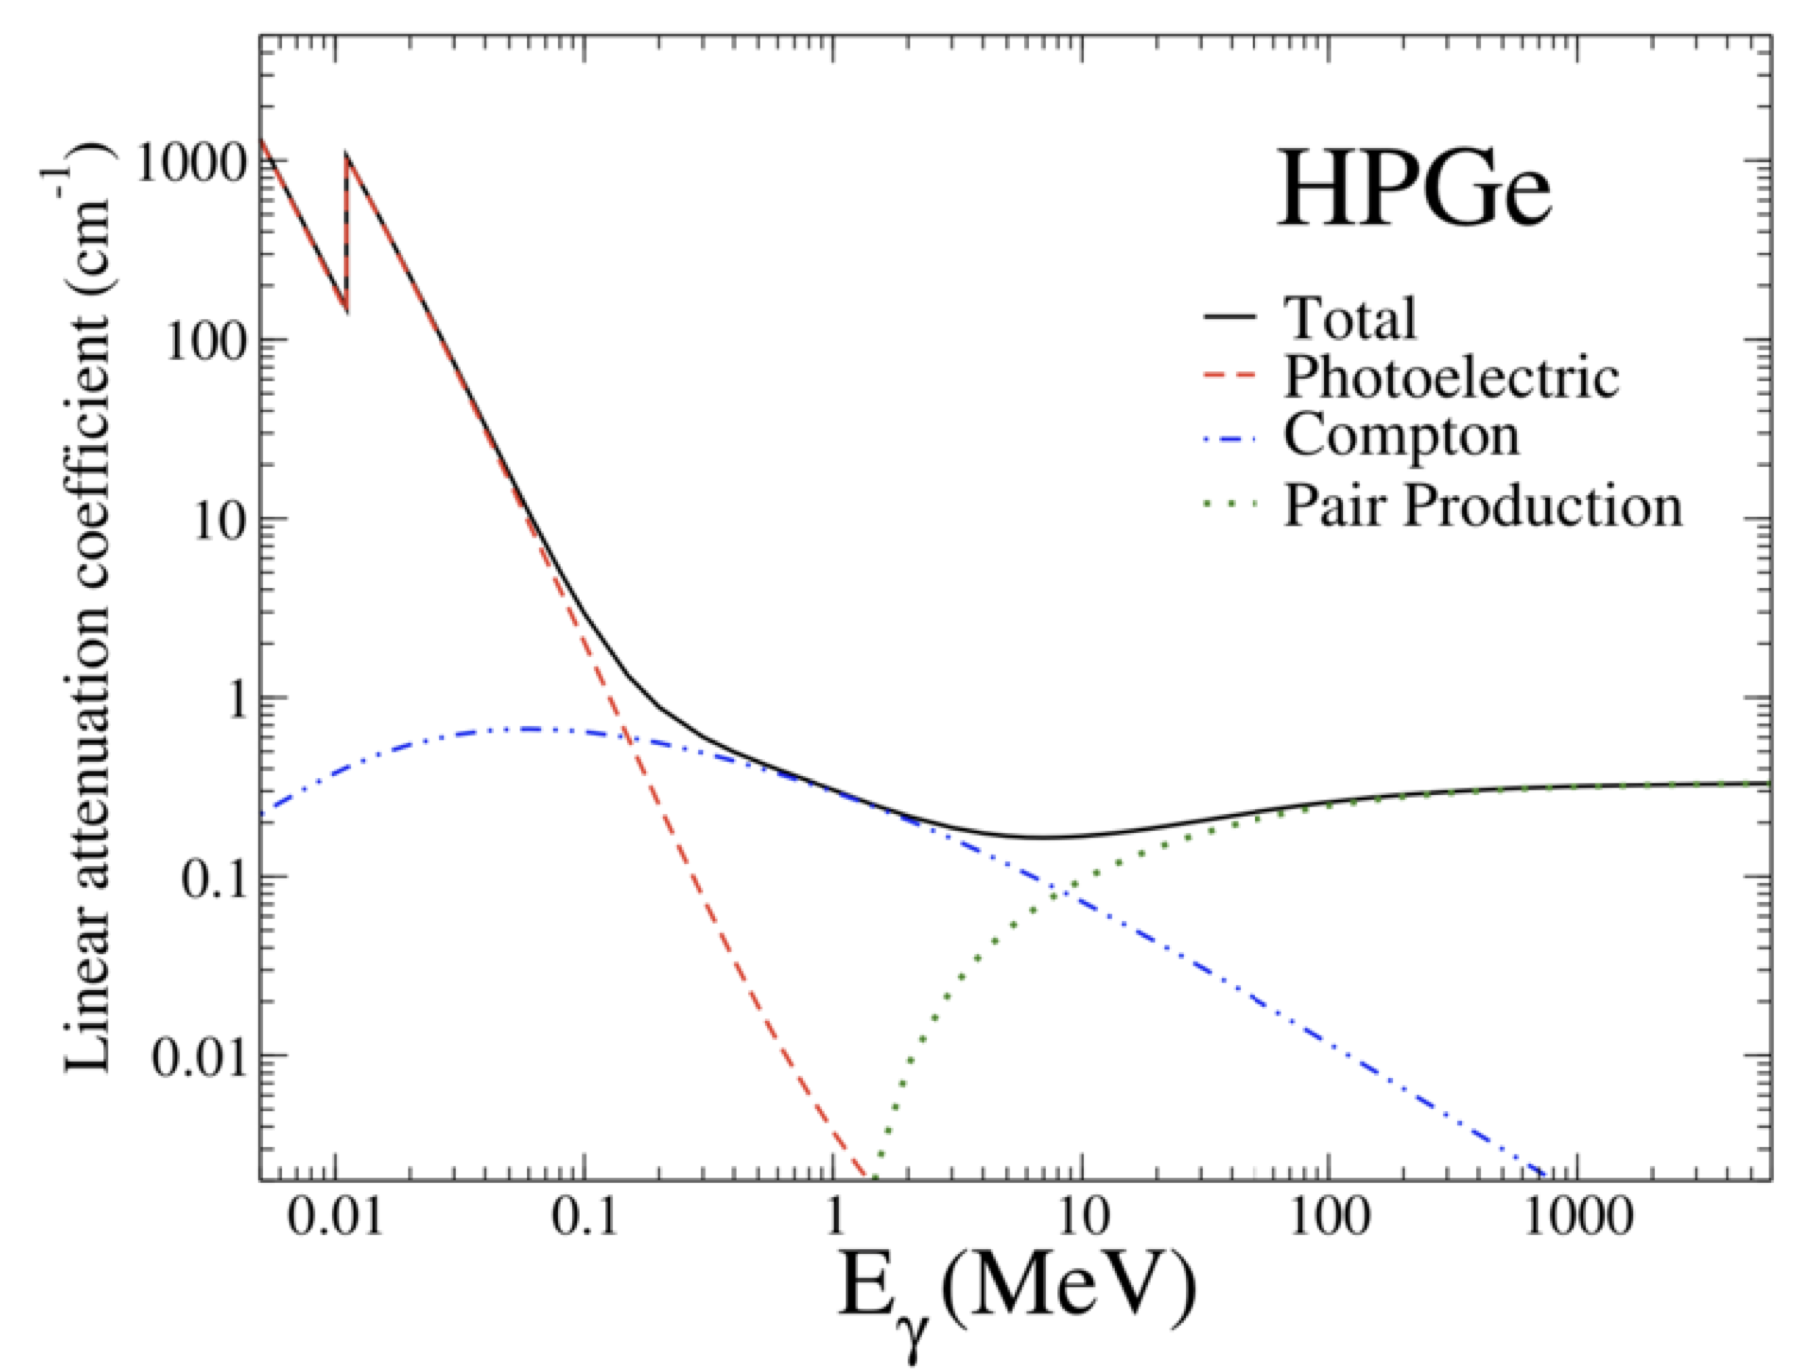
\includegraphics[width=0.95\textwidth]{total_gamma_crosssection.png}
    \caption{The linear attenuation coefficent as a function of $\gamma$-ray energy with individual components for photoelectric absorption, Compton-scattering, and pair production plotted. Figure from~\cite{maclean_spectroscopy_2021}.}
    \label{fig:total_crosssection}
\end{figure}

%------------------------------------------
\subsubsection{Compton-Scattering}
\label{sec:compton_scatter}
%------------------------------------------

Compton scattering takes place when a photon interacts with an atomic electron and is deflected while transferring a portion of its energy to the election. 
This transfer of energy ejects the electron from the nucleus and the $\gamma$-ray is scattered maintaining a fraction of its original energy. 
The energy of the scattered photon, $E^{'}$, can be related to its original energy, $E$, and the scattering angle, $\theta$, via the following:

\begin{equation}
    E^{'} = \frac{E}{1 + \frac{E}{m_e c^2}(1 - \cos(\theta))}
\end{equation}

where $m_e$ is the mass of the electron and $c$ is the speed of light. 


%------------------------------------------
\end{document}
%------------------------------------------